\documentclass{article}
\usepackage{amsmath, amssymb, graphicx, listings, xcolor}
\usepackage{geometry}
\usepackage{float}
\usepackage{minted}
\title{Sinusoidal Time Embedding Explanation and Implementation}
\date{}
\begin{document}

\maketitle

\section{Mathematical Formulation}

Given a scalar timestep $t \in \mathbb{R}$ and an embedding dimension $d \in \mathbb{N}$ (where $d$ is even), the sinusoidal time embedding is computed using alternating sine and cosine functions applied at exponentially scaled frequencies. The output is a vector $\mathbf{e}_t \in \mathbb{R}^d$ defined as:


\[ e_t [2i] = \sin \left( \frac{t}{10000^{2i/d}} \right) \]
\[ e_t [2i+1] = \cos \left( \frac{t}{10000^{2i/d}} \right) \]

for $i = 0, 1, \dots, \frac{d}{2} - 1$.

This allows to encode continuous, smooth representations of time.


\begin{figure}[H]
    \centering
    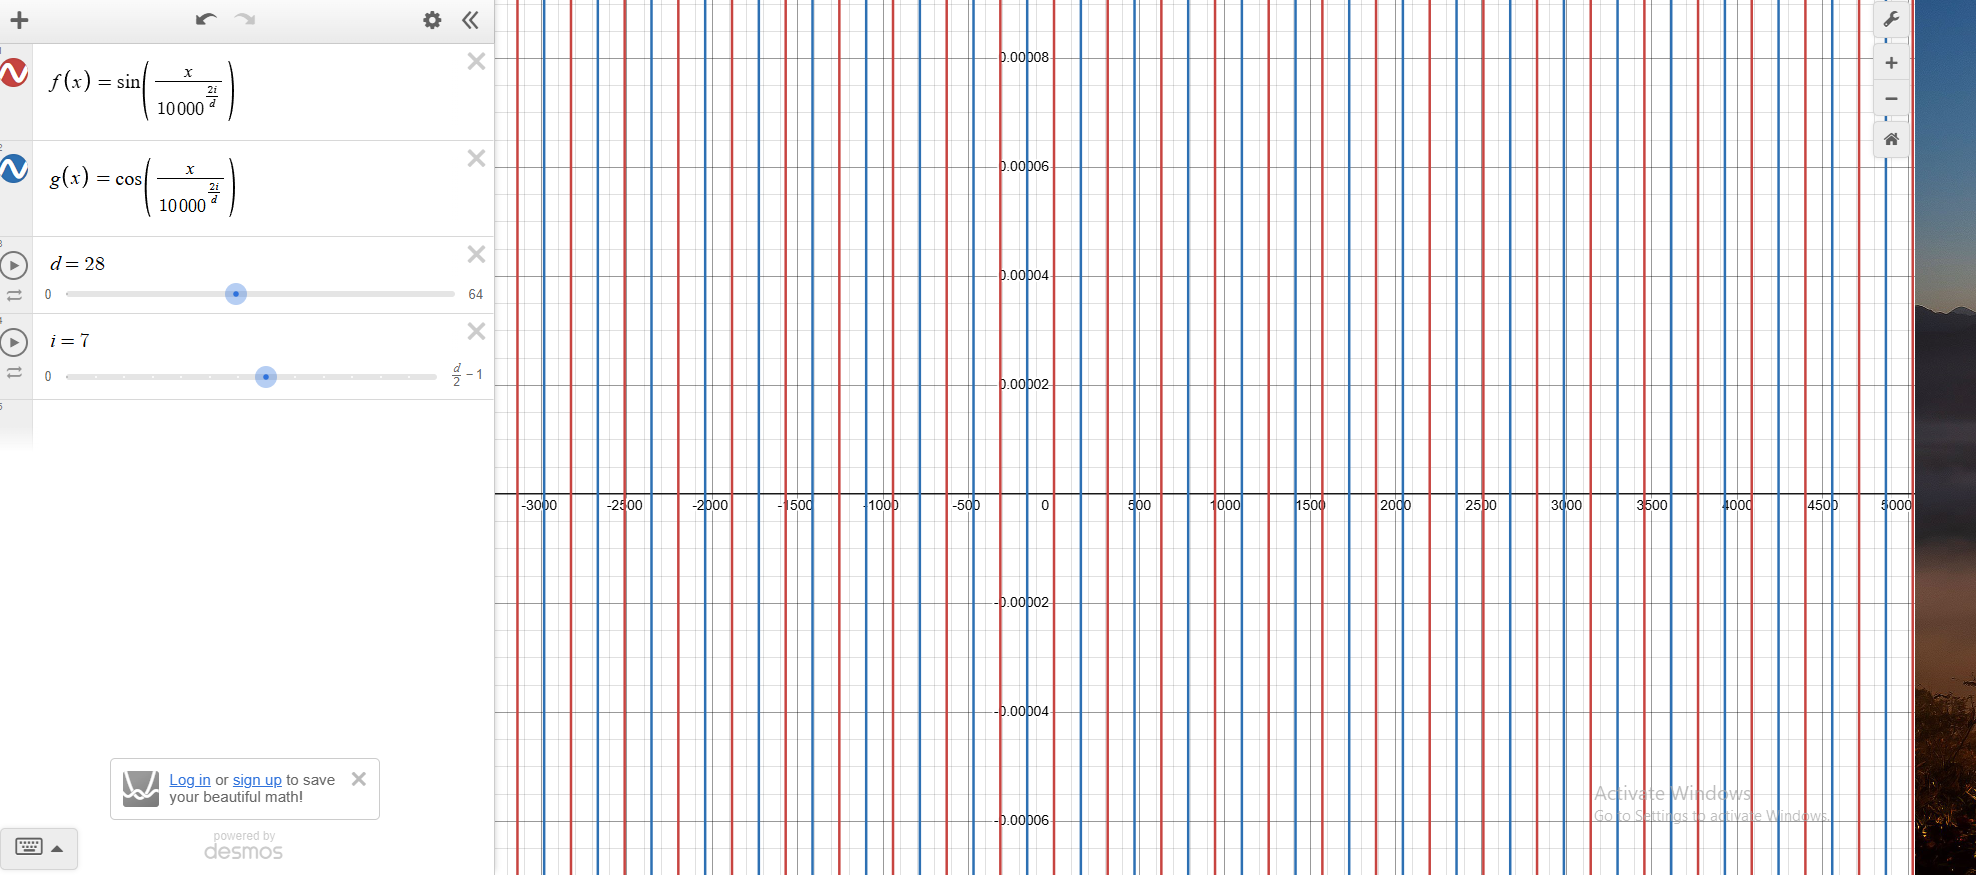
\includegraphics[width=0.8\textwidth]{desmos.png}
    \caption{Cool desmos graph of the above functions.}
\end{figure}


\section{Explanation}

\begin{itemize}
    \item The embedding uses a fixed, non-learned set of sinusoidal functions (compared to other methods where we use machine learning and fully-connected layers to learn the representation of time embeddings).
    \item Even indices (0, 2, 4, ...) use the sine function.
    \item Odd indices (1, 3, 5, ...) use the cosine function.
\end{itemize}

\section{PyTorch Implementation}

\begin{minted}[fontsize=\small, linenos]{python}
# My version
def get_time_embeddings(timesteps: torch.Tensor, embedding_dim: int) -> torch.Tensor:
    assert embedding_dim % 2 == 0, "embedding_dim must be even"

    # Create the frequency spectrum
    half_dim = embedding_dim // 2
    exponent = -math.log(10000.0) / (half_dim - 1)
    freq = torch.exp(torch.arange(half_dim, dtype=torch.float32) * exponent)

    # Expand timesteps for broadcasting
    timesteps = timesteps.float().unsqueeze(1)  # (N, 1)
    args = timesteps * freq.unsqueeze(0)        # (N, half_dim)

    # Concatenate sin and cos
    embedding = torch.cat([torch.sin(args), torch.cos(args)], dim=1)  # (N, embedding_dim)

    return embedding
\end{minted}






\end{document}
